\chapter{Projektgennemførelse}\label{kapitel_Projektgennemforelse}
i dette afsnit beskrives redskaberne gruppen har anvendt i projektgennemførslen blive beskrevet. 

\section{Gruppedannelse}
Gruppen består af Mathias Siig Nørregaard fra IKT, Marie Kirkegaard fra ST og Charlotte Søgaard Kristensen fra ST. 

Gruppensammensætningen er lavet på baggrund af, at projektet omhandler en undersøgelse af, om en automatiseret ultralydsscanner kan udvikles. Gruppen består derfor af én IKT-studerende til udvikling af software, og to ST-studerende til at lave analyser af, hvordan systemet skal opbygges ift. krav fra lovgivning og personale m.m. 

Gruppen blev ved projektstart enige om at finde en reviewgruppe til feedback af gruppens arbejde og omvendt. Reviewgruppen består af Jonas Bæch (ST) og Kathrine Duus Kinnerup (ST), med lektor Samuel Alberg Thrysøe som vejleder. Det har fungeret godt at have en reviewgruppe, da reviewgruppen havde forslag til forbedring af bachelorprojektet.  

\section{Samarbejdsaftale}
Ikke alle gruppemedlemmerne kendte hinanden ved projektstart, og det var derfor vigtigt at få lavet en udførlig samarbejdsaftale som dokumentation for gruppens beslutninger og aftaler, samt rettesnor, hvis der skulle opstå problemer i samarbejdet. 

Det har ikke været nødvendigt at finde samarbejdsaftalen frem, til konflikthåndtering, under projektforløbet, da der ingen problemer har været med samarbejdet. Samarbejdsaftalen er derfor blevet brugt til forventningsafstemning af projektarbejdet samt til at diskutere forventninger og ønsker til projektarbejdet, imellem gruppens medlemmer. 

Samarbejdsaftalen har været et vigtigt redskab for gruppen, da den kan have været medvirkende til at problemerne i samarbejdet aldrig er opstået. Samarbejdesaftalen er vedlagt i bilag \ref{Samarbejdsaftale}. 

\section{Arbejdsfordeling}
Arbejdsfordelingen har fungeret godt, da gruppens medlemmer har haft hvert deres ansvarsområder, hvor arbejdsfordelingen har været opdelt efter kompetencer og interesse hos gruppens medlemmer, samt hvad gruppens medlemmer kunne tænke sig at arbejde med i fremtiden.  

Mathias har primært haft ansvaret for kodningen af software til systemet. Marie og Charlotte har sammen stået for rapportskrivning og brugerundersøgelser, samt risikovurdering af projektet. Marie har haft ansvaret for udarbejdelsen af den medicinske godkendelse, mens Charlotte har haft ansvaret for den overordnede projektstyring og den økonomiske analyse. 

Kravspecifikation, accepttest og design af systemet er diskuteret og udarbejdet i fællesskab, så alle gruppens medlemmer var indforstået med systemets krav og design. 

Da bachelorprojektet er undersøgelsesprojekt, har gruppens medlemmer ind i mellem været udfordret, da mange af opgaverne i projektarbejder var nyt stof for alle. Her har gruppens medlemmer været gode til at hjælpe og spare med hinanden, samt søge hjælp hos vejleder og andre sparringspartnere.  

Nedenstående tabel viser fordelingen af ansvarsområder i gruppen. 

\begin{table}[h]
\centering
\begin{tabular}{|l| p{0.15\textwidth}|}
\hline
\textbf{Ansvarsområde} &  \textbf{Ansvarlig} \\\hline
Kravspecifikation og Accepttest & Fælles \\\hline
Udviklingsdokument & MSN, CSK\\\hline
Brugerundersøgelse & MK, CSK \\\hline
Udvikling af software & MSN\\\hline
Medicinsk godkendelse & MK \\\hline
Overordnet projektstyring & CSK \\\hline
Økonomisk og omkostningseffektiv analyse & CSK \\\hline
\end{tabular}
\caption{Ansvarsområder}
\end{table}

\section{Risikohåndtering af projektarbejdet}
Formålet med risikohåndteringen af projektarbejdet, er at identificere, analysere og evaluere på de risici, der kan opstå under arbejdet med bachelorprojektet. Risikohåndteringen er anvendt som beslutningsgrundlag for planlægning og prioritering af tasks i sprints. Først blev risiciene identificeret, ved brainstorming. Der blev fundet risici inden for softwaren, hardwaren, sociale risici i forhold til gruppearbejdet, generelle projektrisici og risici indenfor de metoder, der er anvendt i projektarbejdet. Derefter blev konsekvensen og sandsynligheden for det enkelte risici vil opstå, stillet op. Konsekvenskriterierne blev beskrevet fra ubetydelig til ødelæggende, og sandsynligheden fra meget usandsynligt til meget sandsynligt. Risikoniveauet for de enkelte risici blev analyseret, og der blev set på konsekvensen af, at ricisien vil opstå og sandsynligheden for at risiciene opstår. Et højt risikoniveau er, at konsekvensen er ødelæggende og sandsynligheden er meget sandsynligt. Risci blev formuleret til tasks. Da man ikke kan ændre på konsekvensen af noget opstår, er tasks blev prioriteret efter konsekvensen. De tasks der havde størst konsekvens og derved ville ødelægge projektet eller forhindre andre tasks i at blive færdige, blev prioriteret først. Risikohåndteringen er kun blevet brugt i forhold til udviklingen af software, da der i udviklingsprocessen har været flest opgaver der har afhængt af hinanden.

\section{Planlægning}
Ved projektstart blev der lavet en standard sekventiel tidsplan. Se bilag \ref{Tidsplan} Tidsplan. Denne tidsplan blev dog hurtigt droppet, da det var umuligt at planlægge sig ud af de alle udfordringer, som implementeringen ville give. Gruppen valgte i stedet at bruge Scrum som projektstyringsværktøj. Scrum blev valgt, da mange faser og tasks i projektet var ukendte, og det var derfor vigtigt at benytte et agilt værktøj gennem projektperioden, hvor gruppen kunne vende tilbage til de enkelte faser og tasks. Den oprindelige tidsplan ville virke bedre for et velkendt system, der skulle implementeres. Gruppen påbegyndte derfor implementeringen hurtigere end tidsplanens oversigt. De overordnede faser fra tidsplanen, lavet ud fra v-modellen, blev stadig forsøgt at blive overholdt, så det passede med reviewgruppens faser. Dette var for eksempel færdiggørelse af kravspecifikation og accepttest. 

\section{Projektledelse}
Der har ikke været en officiel projektleder i gruppen, da gruppen blev vurderet for lille til at have en Scrum-master. Vigtige beslutninger er derfor taget kollektivt. Senere i forløbet blev det dog klart, at én i gruppen, var nødt til at have et overordnet overblik over projektforløbet. Dette blev Charlotte, som: 
\begin{itemize}
\item lavede udkast til sprints  med input fra alle gruppens medlemmer
\item havde overblik over hvilke elementer, der manglede i projektet
\item havde ansvaret for burn-down charts, der giver en indikation af forløbet af sprintet
\end{itemize} 

\section{Projektadministration}
Git, med SourceTree som interface, er blevet anvendt til versionsstyring af projektets dokumenter og kildekode. Dette gjorde, at det var let at se ændringer, finde frem til en tidligere version og håndtere merging, fusionering af dokumenter.

Intern kommunikation i gruppen, har det hovedsageligt foregået verbalt. Når det har været nødvendigt at skrive sammen, har det foregået via Facebooks Messenger-funktion. Ekstern kommunikation med vejleder Michael Alrøe og andre personer, som har hjulpet med projektet, er foregået over e-mail eller telefon. Se bilag \ref{Mails} Mails.  

Hver dag er dagens arbejde skrevet i en logbog. Samtlige færdiggjorte og igangsatte tasks, samt gruppens aftaler er blevet skrevet heri. Logbogen har hjulpet gruppen til at kunne finde tilbage til tidligere aftaler, samt huske hvor en task var blevet pauset. Se bilag \ref{Logbog} Logbog.  

Websiden Trello er anvendt som scrumboard. Hvert Trello-board er et sprint, hvor listerne indeholder Backlog, Ongoing, Stalled, Review og Done. Trello har givet et godt overblik over de enkelte sprints og gruppens medlemmer har hele tiden kunne følge med i hvilke tasks som var i gang, hvem som lavede dem, hvilke tasks der var gået i stå og hvilke tasks der var færdige. Efter sprint 5, blev færdiggjorte tasks opdateret på burn-down chart, til at følge processen i sprintet. 

Nedenstående figur \ref{Trello} viser, hvordan Trello er brugt som Scrumboard til sprint 6. 

\begin{figure}[H]
    \centering
    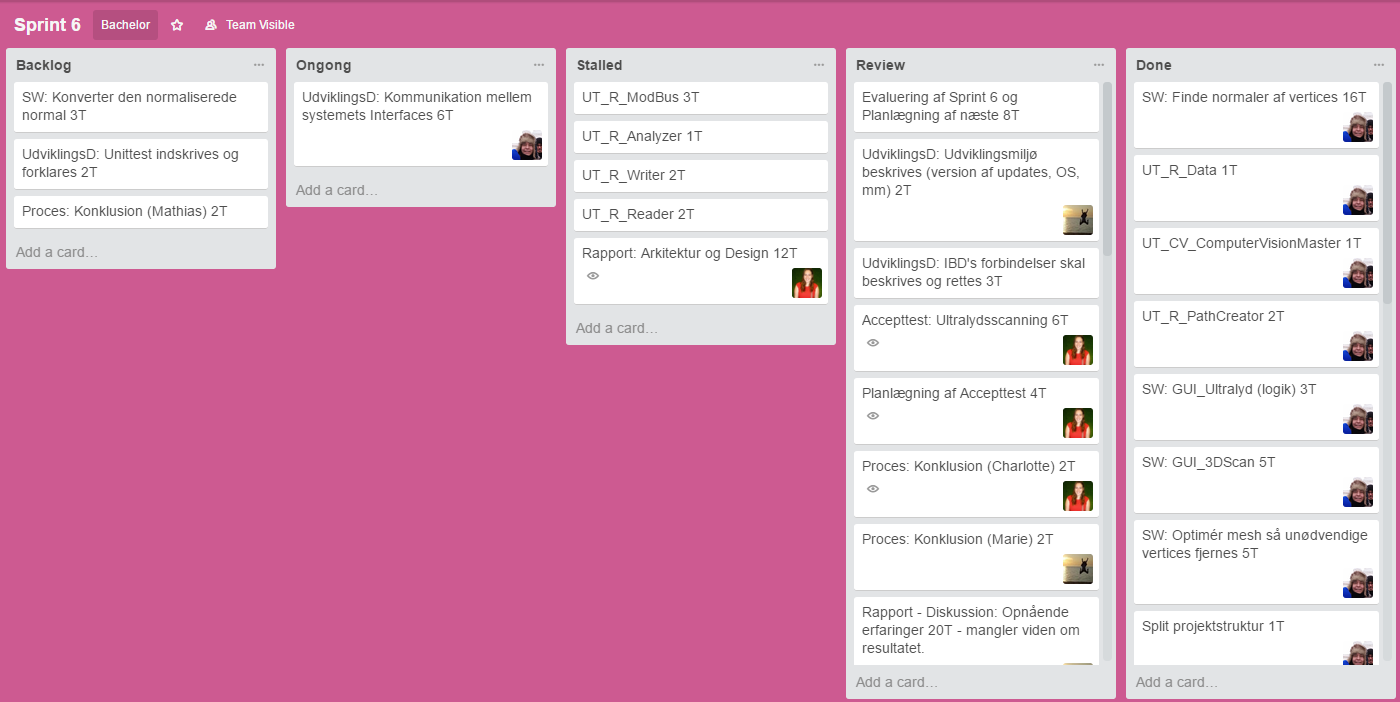
\includegraphics[width=0.35\textwidth]{figurer/d/Trello}
    \caption{Brystets opbygning \citep{Trello}}
    \label{Trello som Scrumboard af sprint 6}
\end{figure}

Nedenstående figur \ref{Burn-down} viser forløbet af sprint 6. Den blå linje er idelle timers arbejde, gruppen skal nå hver dag, og den orange er hvor mange timers arbejde, der blev færdiggjort. 

\begin{figure}[H]
    \centering
    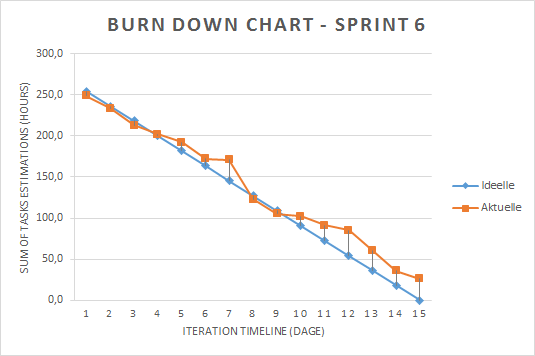
\includegraphics[width=0.35\textwidth]{figurer/d/Burn-down}
    \caption{Brystets opbygning \citep{Burn-down}}
    \label{Burn-down chart for sprint 6}
\end{figure}

\newpage

\section{Udviklingsforløb af koden}
Udviklingen af koden er sket i flere 'steps' ift. risikoanalysen af projektet, se bilag \ref{Risikovurdering} Risikovurdering. Dette er også gjort for løbende at få et Minimum Viable Product (MVP) af kontinuerlig højere kvalitet. 
Ud fra risikoanalysen bilag \ref{Risikovurdering}, blev det vurderet, at følgende 'steps' var vigtigst:

\begin{table}[h]
\centering
\begin{tabular}{|l| p{0.2\textwidth}|}
\hline
\textbf{Step} &  \textbf{Vigtighed} \\\hline
	Kommunikation med UR10 & Meget vigtigt \\\hline
	3D scan output fra Kinect & Meget vigtigt\\\hline
	Find sti af positioner fra 3D scan & Vigtigt \\\hline
	3D output behandling & Vigtigt \\\hline
	Beregn rotationer af fundne positioner & Mindre vigtigt \\\hline
\end{tabular}
\caption{Steps til udvikling af produkt}
\end{table}

Vigtigheden skal forstås sådan, at de mindre vigtige opgaver afhænger af de mere vigtige opgaver. 
Det vil sige, at gruppen har prioriteret at udvikle de vigtige opgaver først, så det til de næste sprints har været nemmere at vurdere tiden, der skulle afsættes for at gennemføre de næste steps.
 
\section{Udviklingsforløb} \label{Udviklingsforlob}
Der var taget udgangspunkt i V-modellen til at nå alle faser i projektarbejdet. Faserene var kravspecifikation, accepttest, design, implementering og test, og de stemte overens med reviewgruppens, sådan at de vigtigste udkast af dokumenter som kravspecifikation og accepttest kunne blive reviewet samtidigt. Tidsplanen, lavet ud fra V-modellen, indeholdte deadlines for, hvornår de forskellige fasers udkast skulle være færdiggjorte, men der var ingen tidsrammer for, hvor lang tid hver task i fasen måtte tage. Derfor besluttede gruppen også at anvende Scrum til at få struktur og styring på bachelorprojektets arbejdsopgaver.

I bachelorprojektet blev der anvendt en modificeret udgave af Scrum, hvor kun delelementer er benyttet. Projektet blev udarbejdet af tre medlemmer, hvilket har betydet, at der ikke har været en Scrum Master, og alle medlemmer har haft ansvar for processen. Product Owner kommer tættest på at være Søren Pallesen fra Robotic Ultrasound, men grundet arbejdstider er Product Owner fravalgt i denne proces. Søren Pallesen har haft rollen som sparringspartner gennem udviklingsperioden, hvor der i alt har været tre møder med ham. Se bilag \ref{Eksterne moder} Eksterne møder. 

Prioriteringen af tasks, til de forskellige sprints, har taget udgangspunkt i risikovurderingen der blev lavet i starten af projektperioden. Her blev det vurderet, hvad der kunne går galt samt konsekvensen af og sandsynligheden for, at det ville gå galt. De tasks med høj risikoprofil, blev prioriteret først i projektarbejdet for at undgå blokader i projektet. Se bilag \ref{Risikovurdering} Risikovurdering.  

Websiden Trello er anvendt til at holde styr på de forskellige tasks. Hvert sprint har sit eget board. Hvert board er delt op i lister; Backlog, Ongoing, Stalled, Review og Done. Ved start af hvert sprint, er de forskellige tasks timesat og skrevet ind i Backlog. Den samlede timebestemmelse til hvert sprint blev udregnet ved at se, hvor meget tid hvert medlem havde til rådighed udover tid til andre studierelaterede opgaver. 

Efter hvert endt forløb er sprintet evalueret og et nyt er blevet planlagt. I de første 4-5 sprints havde alle gruppens medlemmer undervisning, hvilket har præget, hvordan sprints blev planlagt. Det betød, at nogle tidsbestemmelser ikke var præcise, da det til tider var meget svært at vurdere, hvor meget af gruppens tid der skulle afsættes til øvrige fag - specielt under eksamensperioden. Det gav først mening at tage burn-down charts i brug omkring sprint 5, da gruppen på det tidspunkt var blevet meget bedre til at estimere tasks.

Alle backloggens tasks var indskrevet i excel, og ved færdiggørelse af en task, blev datoen noteret, og dokumentet opdaterede automatisk burn-down chart, så man kunne se, hvordan processen lå i forhold til den lineære kurve. Se bilag \ref{Timebestemt sprints} Timebestemt sprints. 

Scrum er kun anvendt frem til den 9. december, da gruppen besluttede, at det ikke gav mening at tidssætte gennemlæsning af de udviklede dokumenter. Den sidste uge blev brugt på gennemlæsning, ensretning og færdigudvikling af dokumentationen for projektet.  

\subsection{Evaluering af de enkelte sprints} 
Dette afsnit vil kort opsummere de vigtigste punkter de forskellige sprints. Det har generelt været svært at timelægge ting, som man ikke har erfaring med - dette vil være en naturlig forhindring i et undersøgelsesprojekt. Den fulde evaluering af Scrum kan ses i bilag \ref{Evaluering Scrum} Evaluering af Scrum.

Der har i projektforløbet været syv sprints, hvor gruppen for hvert sprint er blevet bedre til at strukturere arbejdet og timebestemme de forskellige tasks. Det første sprint var kort og blev primært brugt til klargøring af projektet og undersøgelse af projekts indhold. Det var først midt i første sprint, at Scrum blev indført, hvor havde gruppen indtil anvendt en sekventiel tidsplan og enkelte opgaver var ikke timebestemte. Ved andet sprint blev det forsøgt at timebestemme de forskellige tasks, men ved de tidligere sprint, endte flere tasks i kategorien ”stalled”, grundet at tasks var defineret for bredt. Det blev derfor forsøgt at definere task med målbare resultater, så det blev muligt at afslutte dem. Undervejs har det været nødvendigt at forlænge enkelte sprints, da gruppens medlemmer havde travlt med eksamen. Gruppen blev bedre til at fuldende og timesætte task, men der var stadig problemer med task til implementering. 

Efter sprint fem, blev der lavet et brun-down chart, og det blev efterfølgende besluttet at opdatere Burn-down charts dagligt for at få overblik over sprintenes forløb. Gruppen var blevet bedre til at timebestemme hver task, men oplevede et problem med tasks, der var for store. På baggrund af den erfaring, blev det besluttet at et task max måtte fylde otte timer. Det sidste sprint blev brug for at få alle løse ender samlet. Gruppen besluttede at stoppe udviklingen og dermed brugen af Scrum d. 9 december. Dette blev besluttet for at bruge den sidste uge på review, hvor agil udvikling ikke længere var nødvendig. 
 
\section{Møder}
Vejledermøder har været planlagt efter behov, hvor hvert møde typisk har haft en varighed af 1 time. Gruppen har sendt en dagsorden til vejleder inden hvert møde, og der er skrevet referat til hvert vejledermøde. Se bilag \ref{Vejledermoder} Vejledermøder.
 
Der har i projektperioden været møder med CEO Søren Pallesen, radiolog og ultralydsekspert Lars Bolvig, samt lektor Samuel Alberg Thrysøe. Møder med Søren Pallesen har omhandlet brugen af ultralyd og det fremtidige perspektiv med systemet. Mødet med Samuel Thrysøe har omhandlet spørgsmål til, hvordan specifikke tests af systemet kunne udføres ved brug af et 3D printet bryst. Møderne med Lars Bolvig har omhandlet teknisk viden omkring utralydsundersøgelser. Se bilag \ref{Eksterne moder} Eksterne møder og bilag \ref{Telefoninterview} Interview med radiolog Lars Bolvig. 

\section{Konflikthåndtering}
Samarbejdsaftalen, se bilag \ref{Samarbejdsaftale}, har været et redskab i forebyggelsen af konflikter. Der har i løbet af projektarbejdet ikke været nogle alvorlige konflikter. De uenigheder, der var opstået, blev løst gennem god kommunikation, samt forståelse og gensidig respekt for hinandens synspunkter. Uenighederne har typisk omhandlet, hvordan en specifik task eller lignende skulle løses eller beskrives i rapporten. Hvis det har været nødvendigt at inddrage alle gruppens medlemmer, for at nå til enighed, var det flertallet, der bestemte løsningen. Gruppemedlemmerne er altid nået frem til en løsning, som hele gruppen var indforstået med.

\section{Opnåede erfaringer}
I løbet af projektperioden har gruppen opnået erfaringer inden for agil udvikling, tværfagligt gruppearbejde, kravspecifikation, testspecificering samt dokumentering af et produkt.

Gruppen har opnået erfaring med Scrum som processtyring. Især timebestemmelsen og definering af hvert task, er gruppens medlemmer gradvist blevet bedre til i løbet af hvert sprint. Derudover har gruppen også opnået erfaring med at prioritere tasks til sprints, hvilket er gjort ved brug af risikoanalysen af projektet. Risikoanalysen har dog ikke kunne bruges i alle tilfælde, da den blev lavet før gruppen kendte til alle projektets tasks. Derfor er risikoanalysen mest blevet anvendt til prioriteringen af tasks i softwareudviklingen, da gruppen kunne prioritere, hvilke funktionaliteter de fandt vigtigst for Automatisk Ultralydsscanner. 

Gruppen har også opnået erfaringer i formuleringen og defineringen af tests til accepttest. Gruppen havde problemer med at få UC3: Hovedscenarie testet. Der blev brugt lang tid på at udtænke en test, som kunne teste Robotarms evne til at bevæge sig i et bestemt bevægelsesmønster. Gruppen prøvede at teste bevægelsesmønsteret ved at teste med maling, tape og tucsh, samt beklæde testobjektet med ler, for at kunne se Robotarms bevægelsesmønster. 

Derudover har alle gruppens medlemmer opnået vigtig erfaring med tværfagligt samarbejde med personer, man aldrig har arbejder sammen med før, hvilket er meget virkelighedsnært i forhold til et kommende arbejde i erhvervslivet.
Nedenfor har hvert gruppemedlem beskrevet deres opnåede erfaringer med projektarbejdet. 

\subsection{Charlotte}
Charlotte har i bachelorforløbet fået et større kendskab til projektdokumentation, brugerundersøgelser, økonomi og projektstyring. Charlotte er blevet bedre til LaTeX redigering i løbet af projektet, men hun har har specielt øget sit kendskab til arbejdet med Scrum som projektstyringsværktøj og burn-down chart til at følge processen. Projektstyringen har givet hende en forståelse for planlægning både på langt og kort sigt i et projekt. Det tværfaglige arbejde i forbindelse med bachelorprojektet har givet hende en virkelighedsnær oplevelse af, hvordan det er at arbejde på tværs af professioner. 

\subsection{Marie}
I bachelorprojektet har Marie lært meget af at lave medicinsk godkendelse af Automatisk Ultralydsscanner. Dette har givet hende et godt kendskab til Medical Device Directive, samt tilhørende standarder. Derudover har det også givet hende en forståelse af, hvor omfattende medicinsk godkendelse er for virksomheder. Arbejdet med bachelorprojektet har samtidigt givet Marie et godt kendskab til anvendelsen af Scrum som projektstyringsredskab, samt erfaring med tværfagligt arbejde med både Mathias og vejleder Michael Alrøe, som ikke kommer fra sundhedsteknologi-uddannelsen og derfor er kommet med andre syn på og tilgange til dokumentation af projektarbejde. Arbejdet med bachelorprojektet har også givet Marie et indblik i at udvikle for en kunde med specifikke ønsker til et produkt. 

\subsection{Mathias}
Mathias har fået endnu bedre kendskab til projektarbejdets processer. Selv om han før har prøvet at arbejde med samtlige af projekt-elementerne (Scrum, kommunikation, tværfaglighed, kravspecifikation, dokumentering osv.) der skulle til for at gennemføre opgaven, føler han, at han nu er blevet stærkere på disse områder. Rent teknisk har han opnået erfaring inden for 3D-model teori, som fx udregning af rotationsvektorer, rumtransformation, mesh beregninger m.m. Mathias fik også bedre kendskab til problematikken bag 3D kameraer og robotarme.

\section{Fremtidig arbejdsproces}
I fremtiden kunne det forbedre projektarbejde, at gruppen blev endnu bedre til at definere de enkelte task i sprintene. Det kunne for eksempel gøres ved at beskrive tasken med et formål og omfanget. Det samme gælder specificering af hvert sprint, så der var et formål med sprintet og en beskrivelse af, hvor langt gruppen forventede at være med delsystemet, når sprintet var afsluttet.

Derudover kunne gruppen have delt tasks op, så hvert task f.eks max var otte timer lang. Gruppen kunne også have haft fordel af at udføre daglige scrum standup møder, da gruppemedlemmer nogle gange har været forvirret over hvad andre i gruppen arbejdede med.

Det havde også været en fordel for gruppen at bruge en continuous integration testing server. Dette kunne gøres for at gennemføre kontinuerlig og automatisk unittesting, og fordi unittesting af samtlige tests kan tage lang tid.